\documentclass{article}

\usepackage{booktabs}
\usepackage{graphicx}
\usepackage[margin=1in]{geometry}

\begin{document}

\begin{center}
{\large Supplementary Material}\\[6pt]
{\bf A Controlled Benchmark for Statistical Detection of Noise-Induced
Transitions in Nonlinear Stochastic Dynamics}
\end{center}

\begin{table}[htbp]
  \centering
  \caption{Supplementary Table S1. Bootstrap confidence intervals for mean F1,
  computed by resampling independent test series.}
  \label{tab:supp-bootstrap-f1-ci}
  \begin{tabular}{lll}
\toprule
Scenario & Method & Mean F1 [95\% CI] \\
\midrule
D=0.5, white & SNHT & 0.725 [0.650, 0.800] \\
D=0.5, white & Chow & 0.645 [0.555, 0.733] \\
D=0.5, white & GRU\_v2 & 0.253 [0.182, 0.329] \\
D=0.5, white & CatBoost & 0.243 [0.175, 0.313] \\
D=0.5, white & LSTM\_v2 & 0.207 [0.144, 0.273] \\
D=1, white & Transformer\_v2 & 0.698 [0.682, 0.714] \\
D=1, white & LSTM\_v2 & 0.675 [0.652, 0.696] \\
D=1, white & GRU\_v2 & 0.651 [0.630, 0.670] \\
D=1, white & CUSUM & 0.534 [0.518, 0.551] \\
D=1, white & CatBoost & 0.479 [0.469, 0.490] \\
D=1, pink & Transformer\_v2 & 0.566 [0.555, 0.577] \\
D=1, pink & GRU\_v2 & 0.551 [0.541, 0.561] \\
D=1, pink & LSTM\_v2 & 0.520 [0.508, 0.530] \\
D=1, pink & CUSUM & 0.402 [0.391, 0.413] \\
D=1, pink & CatBoost & 0.216 [0.209, 0.222] \\
D=1.5, white & Transformer\_v2 & 0.643 [0.631, 0.655] \\
D=1.5, white & LSTM\_v2 & 0.599 [0.586, 0.612] \\
D=1.5, white & CUSUM & 0.595 [0.586, 0.603] \\
D=1.5, white & GRU\_v2 & 0.429 [0.412, 0.446] \\
D=1.5, white & CatBoost & 0.341 [0.334, 0.348] \\
\bottomrule
\end{tabular}

\end{table}

\begin{figure}[htbp]
  \centering
  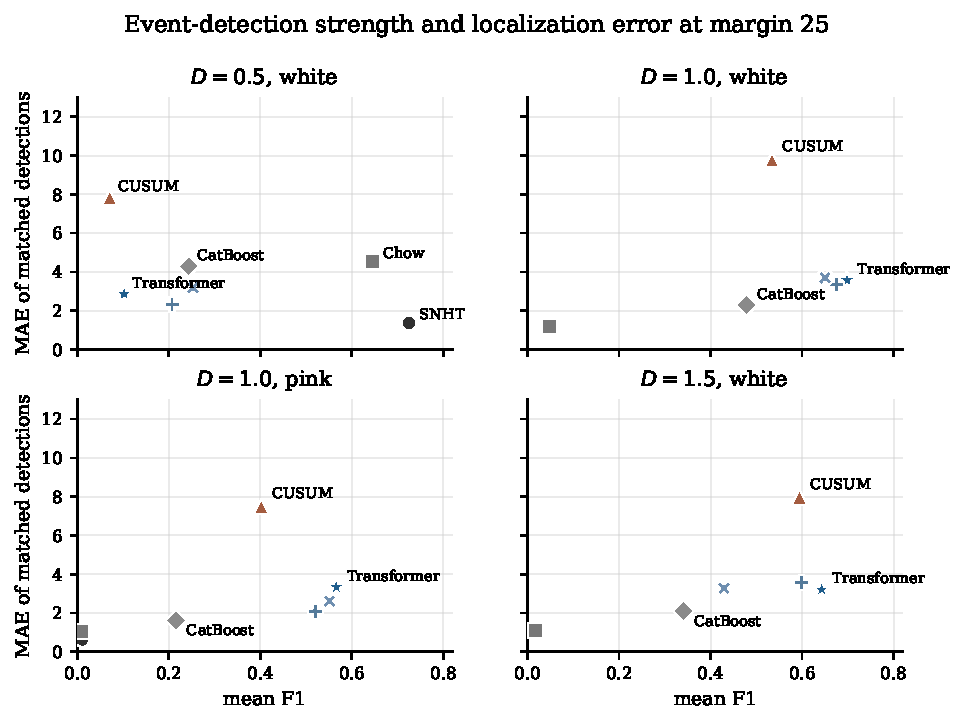
\includegraphics[width=\linewidth]{../assets/figures/fig04_f1_mae_tradeoff.pdf}
  \caption{Supplementary Fig. S1. Mean F1 and mean absolute localization error
  for selected methods at the primary matching margin. MAE is computed only for
  matched detections and should be read together with F1.}
  \label{fig:supp-f1-mae-tradeoff}
\end{figure}

\end{document}
